\chapter{Results}\label{ch:results}

\begin{figure}[H]
\begin{tikzpicture}[
        pc/.style={draw=cyan!80, fill=cyan!5},
        ein/.style={draw=green!80, fill=green!5},
        iin/.style={draw=red!80, fill=red!5},
        pcLabel/.style={font=\small,text=cyan!80},
        einLabel/.style={font=\small,text=green!80},
        iinLabel/.style={font=\small,text=red!80},
        rectNode/.style={draw=black!80, thick},
        roundNode/.style={circle, inner sep=2pt, draw=black!80, thick},
        ]

\pgfdeclarelayer{bg}
\pgfsetlayers{bg,main}
        
 % Nodes
\node[rectNode] (SigmPC) [] {$Sigm$};
\node[rectNode] (SigmEIN) [above left=2cm and 1cm of SigmPC.center]{$Sigm$};
\node[rectNode] (SigmIIN) [below left=2cm and 1cm of SigmPC.center]{$Sigm$};


%% SUBPOPULATIONS FOR EIN
\node[circle, inner sep=1pt, draw, scale=0.3] (out_PSP_PC_e) [right=2.2cm of SigmEIN.east]{};
\draw[-, black!80] (out_PSP_PC_e.west) -- (out_PSP_PC_e.east);
\draw[-, black!80] (out_PSP_PC_e.north) -- (out_PSP_PC_e.south);
\node[circle, draw, thin, inner sep=1pt, above right=0.1cm and 0.15cm of out_PSP_PC_e.center] (PSPPCw1) {\tiny$w_1$};
\node[circle, draw, thin, inner sep=1pt, below right=0.1cm and 0.15cm of out_PSP_PC_e.center] (PSPPCw2) {\tiny$w_2$};
\node[rectNode] (PSPPC1) [right=0.2cm of PSPPCw1.east, thin, inner sep=1pt, fill=white]{\tiny$h_{e_1}(t)$};
\node[rectNode] (PSPPC2) [right=0.2cm of PSPPCw2.east, thin, inner sep=1pt, fill=white]{\tiny$h_{e_2}(t)$};
\node (in_PSP_PC_e) [right=1.38cm of out_PSP_PC_e.center]{};
\node[draw, thick, inner xsep=0.05cm, inner ysep=0.1cm,
      fit=(PSPPC1) (PSPPC2) (PSPPCw1) (PSPPCw2) (in_PSP_PC_e) (out_PSP_PC_e)] (PSPPC) {};


%% SUBPOPULATIONS FOR IIN
\node[circle, inner sep=1pt, draw, scale=0.3] (out_PSP_PC_i) [right=2.2cm of SigmIIN.east]{};
\draw[-, black!80] (out_PSP_PC_i.west) -- (out_PSP_PC_i.east);
\draw[-, black!80] (out_PSP_PC_i.north) -- (out_PSP_PC_i.south);
\node[circle, draw, thin, inner sep=1pt, above right=0.1cm and 0.15cm of out_PSP_PC_i.center] (PSPPCIw1) {\tiny$w_1$};
\node[circle, draw, thin, inner sep=1pt, below right=0.1cm and 0.15cm of out_PSP_PC_i.center] (PSPPCIw2) {\tiny$w_2$};
\node[rectNode] (PSPPCI1) [right=0.2cm of PSPPCIw1.east, thin, inner sep=1pt, fill=white]{\tiny$h_{e_1}(t)$};
\node[rectNode] (PSPPCI2) [right=0.2cm of PSPPCIw2.east, thin, inner sep=1pt, fill=white]{\tiny$h_{e_2}(t)$};
\node (in_PSP_PC_i) [right=1.38cm of out_PSP_PC_i.center]{};
\node[draw, thick, inner xsep=0.05cm, inner ysep=0.1cm,
      fit=(PSPPCI1) (PSPPCI2) (PSPPCIw1) (PSPPCIw2) (in_PSP_PC_i) (out_PSP_PC_i)] (PSPPCI) {};

%% SUBPOPULATIONS FOR PSP_EIN
\node (psp_ein_anchor) [above left= 0.7cm and 3.1cm of SigmPC.west]{};
\node (in_PSP_EIN) [left=0.1cm of psp_ein_anchor)]{};
\node[circle, inner sep=1pt, draw, scale=0.3] (out_PSP_EIN) [right=1.38cm of in_PSP_EIN)]{};
\draw[-, black!80] (out_PSP_EIN.west) -- (out_PSP_EIN.east);
\draw[-, black!80] (out_PSP_EIN.north) -- (out_PSP_EIN.south);
\node[circle, draw, thin, inner sep=1pt, above left=0.1cm and 0.15cm of out_PSP_EIN.center] (PSP_EINw1) {\tiny$w_1$};
\node[circle, draw, thin, inner sep=1pt, below left=0.1cm and 0.15cm of out_PSP_EIN.center] (PSP_EINw2) {\tiny$w_2$};
\node[rectNode] (PSP_EIN1) [left=0.2cm of PSP_EINw1.west, thin, inner sep=1pt, fill=white]{\tiny$h_{e_1}(t)$};
\node[rectNode] (PSP_EIN2) [left=0.2cm of PSP_EINw2.west, thin, inner sep=1pt, fill=white]{\tiny$h_{e_2}(t)$};

\node[draw, thick, inner xsep=0.05cm, inner ysep=0.1cm,
      fit=(PSP_EIN1) (PSP_EIN2) (PSP_EINw1) (PSP_EINw2) (in_PSP_EIN) (out_PSP_EIN)] (PSPEIN) {};

%% SUBPOPULATIONS FOR PSP_IIN
\node (psp_iin_anchor) [below left= 0.7cm and 3.1cm of SigmPC.west]{};
\node (in_PSP_IIN) [left=0.1cm of psp_iin_anchor)]{};
\node[circle, inner sep=1pt, draw, scale=0.3] (out_PSP_IIN) [right=1.38cm of in_PSP_IIN)]{};
\draw[-, black!80] (out_PSP_IIN.west) -- (out_PSP_IIN.east);
\draw[-, black!80] (out_PSP_IIN.north) -- (out_PSP_IIN.south);
\node[circle, draw, thin, inner sep=1pt, above left=0.1cm and 0.15cm of out_PSP_IIN.center] (PSP_IINw1) {\tiny$w_1$};
\node[circle, draw, thin, inner sep=1pt, below left=0.1cm and 0.15cm of out_PSP_IIN.center] (PSP_IINw2) {\tiny$w_2$};
\node[rectNode] (PSP_IIN1) [left=0.2cm of PSP_IINw1.west, thin, inner sep=1pt, fill=white]{\tiny$h_{i_1}(t)$};
\node[rectNode] (PSP_IIN2) [left=0.2cm of PSP_IINw2.west, thin, inner sep=1pt, fill=white]{\tiny$h_{i_2}(t)$};

\node[draw, thick, inner xsep=0.05cm, inner ysep=0.1cm,
      fit=(PSP_IIN1) (PSP_IIN2) (PSP_IINw1) (PSP_IINw2) (in_PSP_IIN) (out_PSP_IIN)] (PSPIIN) {};



\node[rectNode, rounded corners=3mm] (ext) [left=2cm of PSPEIN.west, label={[]:Ext.}]{$p(t)$};
\node (inpIPSP) [left=0.8cm of PSPIIN.west]{};
\node[roundNode] (c1) [above right=0.8cm and 2.5cm of SigmPC.east]{$C_1$};
\node[roundNode] (c2) [left=1cm of SigmEIN.west]{$C_2$};
\node[roundNode] (c3) [below right=0.8cm and 2.5cm of SigmPC.east]{$C_3$};
\node[roundNode] (c4) [left=1cm of SigmIIN.west]{$C_4$};

% add PC
\node[roundNode] (addPC) [left=0.8cm of SigmPC.west]{};
%\draw[-, black!80, thick] (addPC.north west) -- (addPC.south east);
%\draw[-, black!80, thick] (addPC.north east) -- (addPC.south west);
% add Excitatory
\node[roundNode] (addExc) [left=0.8cm of PSPEIN.west]{};
\draw[-, black!80, thick] (addExc.west) -- (addExc.east);
\draw[-, black!80, thick] (addExc.north) -- (addExc.south);

% add PC -> Sigm PC -> PSP PC
\draw[-{Stealth[scale=1.5]}] (addPC.east) -- (SigmPC.west)node[coordinate, pos=0.5](measurepoint){};
\draw[-{Stealth[scale=1.5]}] (SigmPC.east) -| (c1.south);
\draw[-{Stealth[scale=1.5]}] (SigmPC.east) -| (c3.north);


% y0 -> C1 -> Sigm EIN
\draw[-] (c1.north) |- (in_PSP_PC_e.center);
\draw[-{Stealth[scale=0.5]}] (in_PSP_PC_e.center) |- (PSPPC1.east);
\draw[-{Stealth[scale=0.5]}] (in_PSP_PC_e.center) |- (PSPPC2.east);
\draw[-{Stealth[scale=0.5]}] (PSPPC1.west) -- (PSPPCw1.east);
\draw[-{Stealth[scale=0.5]}] (PSPPC2.west) -- (PSPPCw2.east);
\draw[-{Stealth[scale=0.5]}] (PSPPCw1.west) -| (out_PSP_PC_e.north);
\draw[-{Stealth[scale=0.5]}] (PSPPCw2.west) -| (out_PSP_PC_e.south);
\draw[-{Stealth[scale=1.5]}] (out_PSP_PC_e.west) -- (SigmEIN.east) node[pos=0.4, above=0.1cm, fill=pyratesgreen!15,
draw=pyratesgreen, text=pyratesgreen]{\tiny$PSP_{EIN}$};

% y0 -> C3 -> Sigm IIN
\draw[-] (c3.south) |- (in_PSP_PC_i.center);
\draw[-{Stealth[scale=0.5]}] (in_PSP_PC_i.center) |- (PSPPCI1.east);
\draw[-{Stealth[scale=0.5]}] (in_PSP_PC_i.center) |- (PSPPCI2.east);
\draw[-{Stealth[scale=0.5]}] (PSPPCI1.west) -- (PSPPCIw1.east);
\draw[-{Stealth[scale=0.5]}] (PSPPCI2.west) -- (PSPPCIw2.east);
\draw[-{Stealth[scale=0.5]}] (PSPPCIw1.west) -| (out_PSP_PC_i.north);
\draw[-{Stealth[scale=0.5]}] (PSPPCIw2.west) -| (out_PSP_PC_i.south);
\draw[-{Stealth[scale=1.5]}] (out_PSP_PC_i.west) -- (SigmIIN.east) node[pos=0.4, below=0.1cm, draw=pyratesdarkred,
fill=pyratesdarkred!15, text=pyratesdarkred]{\tiny$PSP_{IIN}$};


% Sigm EIN -> c2 -> add EXC
\draw[-{Stealth[scale=1.5]}] (SigmEIN.west) -- (c2.east);
\draw[-{Stealth[scale=1.5]}] (c2.west) -| (addExc.north) node[pos=0.9, right]{\small$+$};
% external -> add EXC
\draw[-{Stealth[scale=1.5]}] (ext.east) -- (addExc.west) node[pos=0.9, above]{\small$+$};

% add EXC -> PSP EIN
\draw[-] (addExc.east) -- (in_PSP_EIN.center);
% inside PSP EIN
\draw[-{Stealth[scale=0.5]}] (in_PSP_EIN.center) |- (PSP_EIN1.west);
\draw[-{Stealth[scale=0.5]}] (in_PSP_EIN.center) |- (PSP_EIN2.west);
\draw[-{Stealth[scale=0.5]}] (PSP_EIN1.east) -- (PSP_EINw1.west);
\draw[-{Stealth[scale=0.5]}] (PSP_EIN2.east) -- (PSP_EINw2.west);
\draw[-{Stealth[scale=0.5]}] (PSP_EINw1.east) -| (out_PSP_EIN.north);
\draw[-{Stealth[scale=0.5]}] (PSP_EINw2.east) -| (out_PSP_EIN.south);
% PSP EIN -> add PC
\draw[-{Stealth[scale=1.5]}, fill=none] (out_PSP_EIN.east) -| (addPC.north) node[pos=1, left]{\small$+$} node[pos=0.4, above=0.1cm, draw=pyratespurple, fill=pyratespurple!15, text=pyratespurple]{\tiny$PSP_{PC_E}$};

% Sigm IIN -> C4 -> PSP IIN
\draw[-{Stealth[scale=1.5]}] (SigmIIN.west) -- (c4.east);
\draw[-] (c4.west) -| (inpIPSP.center);
\draw[-] (inpIPSP.center) -- (in_PSP_IIN.center);
% inside PSP IIN
\draw[-{Stealth[scale=0.5]}] (in_PSP_IIN.center) |- (PSP_IIN1.west);
\draw[-{Stealth[scale=0.5]}] (in_PSP_IIN.center) |- (PSP_IIN2.west);
\draw[-{Stealth[scale=0.5]}] (PSP_IIN1.east) -- (PSP_IINw1.west);
\draw[-{Stealth[scale=0.5]}] (PSP_IIN2.east) -- (PSP_IINw2.west);
\draw[-{Stealth[scale=0.5]}] (PSP_IINw1.east) -| (out_PSP_IIN.north);
\draw[-{Stealth[scale=0.5]}] (PSP_IINw2.east) -| (out_PSP_IIN.south);
% PSP IIN -> add PC
\draw[-{Stealth[scale=1.5]}, fill=none] (out_PSP_IIN.east) -| (addPC.south) node[pos=1, left]{\small$-$} node[pos=0.4, below=0.1cm, draw=pyratesorange, fill=pyratesorange!10, text=pyratesorange]{\tiny$PSP_{PC_I}$};

% electrode
\draw (measurepoint.north) -- (-0.9,1)node[coordinate,pos=0.9](a){} -- (-0.6,0.9)node[coordinate, pos=0.5](b){} -- cycle;
\node (signal)[above right=0.05cm and 2.0cm of a]{\tiny$PSP_{PC}$};
\draw (b.center) |- (signal.west);


%\begin{scope}[shift={(PSPPC1.south west)}]
%      \begin{axis}[yscale=0.03, xscale=0.1,
%            axis x line=none,
%            axis y line=none,
%            domain=0:140,
%            samples=1001,
%            xticklabels=\empty,
%          ]
%          \addplot [green!80] {0.325*x*e^(-0.1*x)};
%        \end{axis}
%\end{scope}
%
%\begin{scope}[shift={(PSPPCI.south west)}]
%      \begin{axis}[yscale=0.03, xscale=0.16,
%            axis x line=none,
%            axis y line=none,
%            domain=0:1400,
%            samples=1001,
%            xticklabels=\empty,
%          ]
%          \addplot [green!80] {0.325*x*e^(-0.1*x)};
%        \end{axis}
%\end{scope}
%
%\begin{scope}[shift={(PSPEIN.south west)}]
%      \begin{axis}[yscale=0.03, xscale=0.16,
%            axis x line=none,
%            axis y line=none,
%            domain=0:140,
%            samples=1001,
%            xticklabels=\empty,
%          ]
%          \addplot [green!80] {0.325*x*e^(-0.1*x)};
%        \end{axis}
%\end{scope}
%
%\begin{scope}[shift={(PSPIIN.south west)}]
%      \begin{axis}[yscale=0.12, xscale=0.16,
%            axis x line=none,
%            axis y line=none,
%            domain=0:140,
%            samples=1001,
%            xticklabels=\empty,
%          ]
%          \addplot [red!80] {1.1*x*e^(-0.05*x)};
%        \end{axis}
%\end{scope}

\begin{pgfonlayer}{bg}

    \node[draw=cyan!40, fill=cyan!2, inner xsep=0.15cm, inner ysep=0.15cm,
      fit=(PSPEIN) (SigmPC) (PSPIIN) ] {};
%    \filldraw [fill=cyan!2,draw=cyan!40]
%        ($ (PSPEIN.center) + (-0.4,0.8) $)
%        rectangle ($ (PSPIIN.center) + (3.8,-0.8) $);
    \node [below=0.2cm of SigmPC, text=cyan]{PC};

    \node[draw=green!40, fill=green!2, inner xsep=0.15cm, inner ysep=0.15cm,
      fit=(PSPPC) (SigmEIN) ] {};
%    \filldraw [fill=green!2,draw=green!40]
%        ($ (SigmEIN.north) + (-0.7,0.4) $)
%        rectangle ($ (PSPPC.south) + (0.4,-0.2) $);
    \node [above=1.4cm of SigmPC, text=green]{EIN};
    
    \node[draw=red!40, fill=red!2, inner xsep=0.15cm, inner ysep=0.15cm,
      fit=(PSPPCI) (SigmIIN) ] {};
%    \filldraw [fill=red!2,draw=red!40]
%        ($ (SigmIIN.north) +  (-0.7,0.2) $)
%        rectangle ($ (PSPPCI.south) + (0.4,-0.4) $);
    \node [below=1.4cm of SigmPC, text=red]{IIN};
\end{pgfonlayer}

\end{tikzpicture}
\caption{\textbf{David \& Friston Block Diagram as implemented in PyRates:}}
\label{fig:pyratesDFBlock}
\end{figure}

\section{General features of the simulated data}\label{sec:general-features-of-the-simulated-data}

The NMM is configured to simulate data with a step-size of $1 ms$, yielding a $1000 Hz$ signal.
In its initial state, the system reacts with high-amplitude oscillations to the "disturbance" of the random input.
However, the signal usually stabilizes quickly and exhibits the expected behaviour.
Thus, the first few seconds (stabilization-time varies with parameterization) of simulated data
are always discarded before further analysis.
When generating data continuously (without re-initialization of the state-variables),
this problem only occurs once in the very beginning.
Changing system parameters abruptly during simulation can also result in disturbances and destabilize the
signal.

\begin{figure}[H]
    \centering
    \begin{tikzpicture}
        \pgfplotsset{
        %% Axis
            scale only axis,
            width=0.4\linewidth,
            height=4cm,
            every axis/.append style={
                line width=1pt,
                tick style={line width=0.8pt},
                %   grid style={dashed, black!20},
                %  grid=major,
            },
%               %% X-Axis
            xmin=-0.1,
            xmax=7,
        }
        \begin{groupplot} [
                group style={
                    group size=2 by 2,
                    vertical sep=12mm,
                    horizontal sep=12mm,
                },
                yticklabel style={
                    /pgf/number format/fixed,
                    /pgf/number format/precision=2
                },
                legend style={nodes={scale=0.8, transform shape}, thin},
                legend image post style={scale=0},
            ]
            \nextgroupplot[ylabel=$mV$, xlabel=$s$]
            \addplot [line width=.5pt,solid, cyan]
            table[x=x,y=y ,col sep=comma]{data/methodology/uncut.csv};
            \legend{\textbf{A)} uncut data};

            \nextgroupplot[xmin=3.0, xlabel=$s$]
            \addplot [line width=.5pt,solid, cyan]
            table[x=x,y=y ,col sep=comma]{data/methodology/uncut.csv};
            \legend{\textbf{B)} cut data};

            \nextgroupplot[xmax=30.0, ylabel=$dB$, xlabel=$Hz$]
            \addplot [line width=.5pt,solid, cyan]
            table[x=x,y=y ,col sep=comma]{data/methodology/psd_welch_jr.csv};
            \legend{\textbf{C)} J-R PSD};

            \nextgroupplot[xmax=30.0, xlabel=$Hz$]
            \addplot [line width=.5pt,solid, cyan]
            table[x=x,y=y ,col sep=comma]{data/methodology/psd_welch_df.csv};
            \legend{\textbf{D)} D\&F PSD};

        \end{groupplot}
    \end{tikzpicture}

    \caption{
        \textbf{Processing of simulated data.} \\
        \textbf{A) \& B):} removing initially unstable signal by cutting off the first $3s$ of the
        data (generated by Simple Jansen-Rit Model with $C=135$.). \\
        \textbf{C) \& D):} Power Spectral Density of Jansen-Rit and David \& Friston Model (Welch's Method)
    }
    \label{fig:initial_oscilations}
\end{figure}

\section{Visualization}\label{sec:visualization}

\begin{figure}[H]
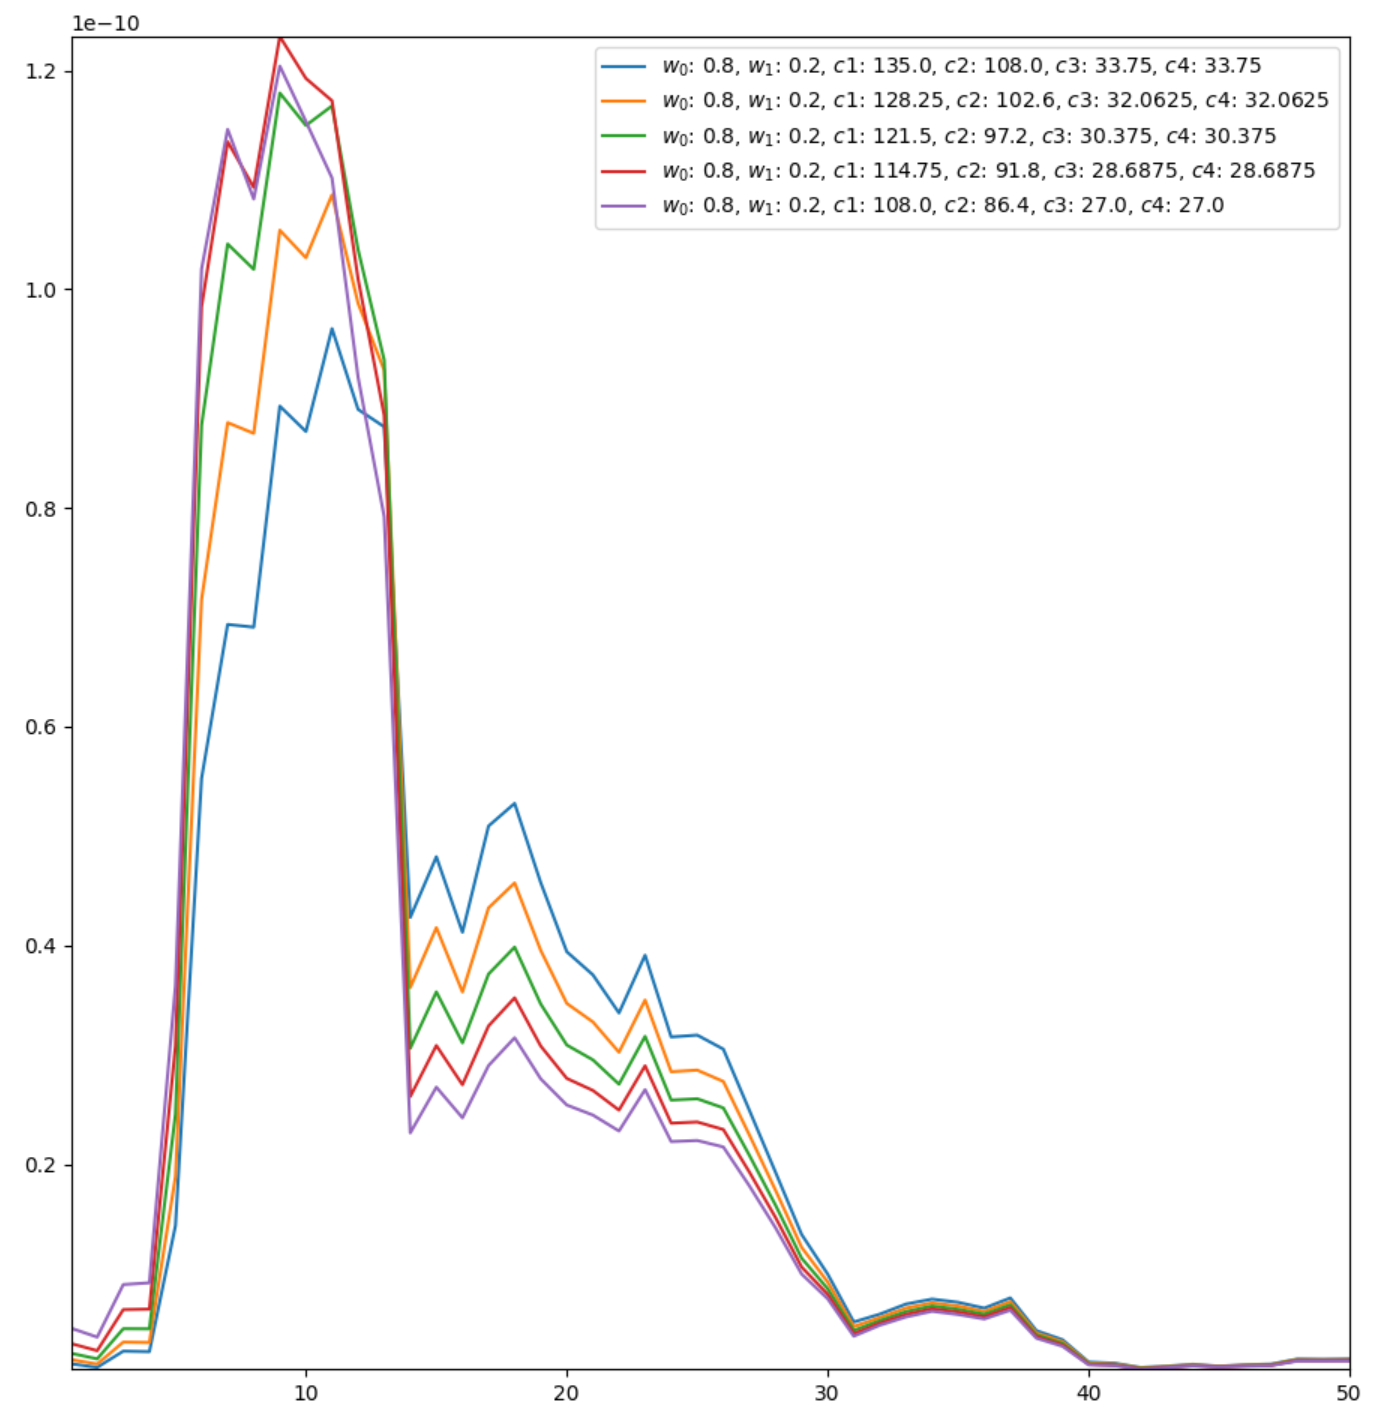
\includegraphics[width=14cm]{Figures/temp_sim_results}
\caption{\textbf{Power Spectral Density of Simulation Results:} Reduction of the connectivity parameter $C$
    from $135$ to $108$ shows a tendency of reducing the strength of the frequency-bands above 12--14Hz,
    while increasing it below that value - especially around 8--12Hz.}
\label{fig:sim_results1}
\end{figure}

\todo{objective description of simulation results}